% !TeX program = xelatex
% UTF-8. Compile twice from this directory:
% xelatex -interaction=nonstopmode -halt-on-error S07_Bao_Cao_RAG_HCMUS.tex
% The figure and equations are native LaTeX; no external assets are required.
\documentclass[12pt,a4paper]{article}
\usepackage[top=1.95cm,bottom=1.95cm,left=2.05cm,right=2.05cm]{geometry}
\usepackage{fontspec}
\IfFontExistsTF{Times New Roman}{\setmainfont{Times New Roman}}{\setmainfont{TeX Gyre Termes}}
\IfFontExistsTF{Arial}{\setsansfont{Arial}}{\setsansfont{TeX Gyre Heros}}
\usepackage{amsmath,amssymb}
\usepackage{array,booktabs,tabularx}
\usepackage{enumitem}
\usepackage{float,caption,needspace}
\usepackage{tikz}
\usetikzlibrary{arrows.meta}
\usepackage{xcolor}
\usepackage{fancyhdr}
\usepackage[unicode]{hyperref}
\definecolor{linkblue}{RGB}{9, 105, 218}
\hypersetup{
  pdftitle={Evaluating Retrieval and Grounding Reliability of RAG in Academic Regulations QA},
  pdfauthor={Bui Trong Tuan Linh (24125066), Tran Dang Le Huy (24125057), Trinh Vo Nam Kiet (24125013)},
  pdfsubject={Empirical Investigation on HCMUS Regulatory Data},
  colorlinks=true,
  linkcolor=linkblue,
  citecolor=linkblue,
  urlcolor=linkblue
}
\renewcommand{\figurename}{Figure}
\renewcommand{\tablename}{Table}
\renewcommand{\refname}{References}
\captionsetup{font=small,labelfont=bf,labelsep=period,skip=4pt}
\pagestyle{fancy}
\fancyhf{}
\fancyfoot[R]{\small CS420 \textperiodcentered{} S07\quad /\quad \thepage}
\renewcommand{\headrulewidth}{0pt}
\renewcommand{\footrulewidth}{0pt}
\setlength{\parindent}{0pt}
\setlength{\parskip}{4.5pt}
\setlength{\tabcolsep}{3.8pt}
\renewcommand{\arraystretch}{1.14}
\linespread{1.05}
\setlength{\emergencystretch}{2em}
\widowpenalty=10000
\clubpenalty=10000
\raggedbottom
\newcommand{\chunkid}[1]{{\footnotesize\nolinkurl{#1}}}
\newcommand{\commitlink}[1]{\href{https://github.com/namkiet/CS420_SeminarRAG/commit/#1}{\textcolor{linkblue}{\textbf{\texttt{#1}}}}}
\begin{document}
\begin{center}
{\LARGE\bfseries Evaluating Retrieval and Grounding Reliability of RAG\\[3pt]
in Academic Regulations Question Answering\par}
\vspace{4pt}
{\itshape An Empirical Study on HCMUS Regulatory Documents\par}
\vspace{5pt}
{\small Bùi Trọng Tuấn Lĩnh (24125066) \textperiodcentered{} Trần Đặng Lê Huy (24125057) \textperiodcentered{} Trịnh Võ Nam Kiệt (24125013)\par}
\vspace{2pt}
{\footnotesize University of Science, Vietnam National University Ho Chi Minh City (VNU-HCM)\par}
\end{center}

\section*{Abstract}

Retrieval-Augmented Generation (RAG) augments large language models with external non-parametric corpora to support knowledge-intensive tasks requiring factual grounding. This paper investigates the empirical relationship between evidence coverage and answer reliability on official academic regulatory documents from VNU-HCM University of Science (HCMUS). The experimental corpus comprises 162 chunks extracted across four regulatory documents (51 pages) alongside a reference benchmark of 20 questions associated with 30 distinct evidence groups. Three retrieval models---TF-IDF, BM25, and dense BGE-M3---are benchmarked at $k \in \{1, 3, 5\}$. BM25 achieves the highest Evidence Recall@1 (80.00\%), whereas BGE-M3 yields the highest Evidence Recall@5 (89.17\%). Generation experiments evaluate 80 candidate answers generated by Qwen2.5-1.5B-Instruct across a no-retrieval baseline and three top-5 RAG configurations. Preliminary GPT-based qualitative review indicates that core factual accuracy improves from 0\% in the unaugmented baseline to 45--50\% under RAG. However, all 60 RAG-generated answers fail to produce valid citation identifiers. Case analyses demonstrate persistent failure modes, notably condition omission and misreading tabular structures, even when gold evidence is present in the prompt context. These empirical findings indicate that while document augmentation substantially enhances response accuracy, it does not eliminate hallucinations, underscoring the necessity of secondary verification and explicit claim-level attribution mechanisms.

\textbf{Keywords} \textperiodcentered{} Retrieval-Augmented Generation, information retrieval, hallucination, academic regulations, evidence attribution.

\section{Introduction}

Question answering within university academic regulations demands both high factual precision and strict adherence to administrative applicability boundaries. Determining graduation criteria, credit transfer policies, or semester tuition fees fundamentally depends on cohort intake years, academic tracks, operational timelines, and exceptions. RAG addresses these constraints by pairing the parametric memory of a generative model with non-parametric documents retrieved dynamically at inference time \cite{ref1}. Nonetheless, necessary evidence can be overlooked during retrieval, obscured by adjacent distractor passages, or misinterpreted by the generator. This raises the central guiding research question: \emph{Does providing external documents eliminate hallucinations in language models?}

This study investigates this guiding question across three systematic dimensions. First, we examine the quantitative impact of retrieval algorithms and cut-off parameter $k$ on evidence coverage. Second, we assess output answer reliability when fixing the generator architecture while varying the provided retrieval context. Third, we trace failure origins by cross-examining evaluation queries, retrieved candidate passages, and generated outputs. The core experimental contributions include: (i) benchmarking three distinct retrieval models on an authoritative regulatory corpus; (ii) evaluating four generation conditions on a frozen instruction-tuned LLM; and (iii) analyzing five traceable failure archetypes. All findings are critically discussed within the scope of our corpus and query benchmarks.

\section{Theoretical Background and Related Work}

\subsection{Parametric and Non-Parametric Memory}

Parametric memory stores knowledge implicitly within the learned weight matrices of a neural language model. In contrast, non-parametric memory provides accessible, external text passages retrieved dynamically at inference time. In a standard RAG workflow, a retrieval component selects relevant candidate passages conditioned on the input query; the generator then conditions its decoding on both the query and these retrieved passages to construct the final response. Retaining passage identifiers within the prompt structure provides an audit trail for factual verification \cite{ref1}.

Fine-tuning updates parametric weights using specialized domain data, steering model behavior and internal knowledge. Providing entire corpora directly into the context window exploits non-parametric memory without retrieval, but incurs severe computational and financial latency that scales with token length. RAG introduces an intermediate retrieval step that filters the external corpus into a bounded top-$k$ context. While this architecture allows modular updates to the knowledge base without retraining, end-to-end response reliability remains strictly bottlenecked by retrieval recall and context utilization.

\subsection{Architectural Foundations of Lewis et al.}

Lewis et al. \cite{ref1} formalized the coordination between a parametric generator and a dense Wikipedia passage index. Their framework employs Dense Passage Retrieval (DPR) to encode queries and documents into latent representations, computing relevance via inner products, coupled with a BART sequence-to-sequence generator. The retrieved document is modeled as a latent variable. Under RAG-Sequence, candidate sequences are marginalized across documents at the full sequence level, whereas RAG-Token marginalizes passage probabilities at each individual token step.

On Natural Questions, Lewis et al. reported Exact Match scores of 44.5 for RAG-Sequence, 44.1 for RAG-Token, and 36.6 for a purely parametric T5-11B+SSM baseline. On WebQuestions, RAG-Token achieved 45.5 while RAG-Sequence reached 45.2, indicating that performance trade-offs vary across benchmark domains. Qualitatively, the authors observed substantially reduced factual errors compared to BART on MS MARCO \cite{ref1}. In our HCMUS setting, we adopt the modern open-weights instruction-tuned Qwen architecture and augment prompt contexts with top-$k$ retrieved chunks to evaluate structured university regulations \cite{ref6}.

\subsection{Answer Verifiability and Attribution}

Schneider \cite{ref2} establishes conceptual requirements for explainability in generative AI (GenXAI), emphasizing that answer verifiability requires linking generated claims directly to grounding evidence. Our study operationalizes this framework across three decoupled evaluation dimensions: retrieval coverage measures the retriever's ability to capture necessary gold evidence chunks; content correctness assesses factual conclusions and administrative applicability conditions; and citation traceability audits passage identifier validity and sentence-level grounding support. Decoupling these dimensions is vital: an answer discussing tuition fees may compute correct numerical amounts while misattributing them to the wrong cohort or column. Conversely, a syntactically valid citation tag may reference an irrelevant paragraph. Rigorous verification must therefore evaluate the triadic relationship between generated proposition, cited passage, and administrative scope. Retaining explicit input-output logs provides the experimental foundation for error decomposition.

\section{Probabilistic Modeling and Numerical Example}

\subsection{Document Marginalization Formulations}

Let $x$ denote an input prompt token sequence, $y = (y_1, \dots, y_T)$ represent a candidate response consisting of $T$ tokens, and $Z$ represent the knowledge corpus. The set $Z_k(x)$ contains up to $k$ candidate chunks with the highest retrieval scores for query $x$. For each position $i \in \{1, \dots, T\}$, $y_i$ is the $i$-th token and $y_{<i}$ represents its preceding prefix sequence. Vector parameters $\eta$ and $\theta$ parameterize the retriever and generator, respectively. Here, $p_\eta(z \mid x)$ denotes the probability of selecting passage $z$, while $p_\theta(y_i \mid x, z, y_{<i})$ denotes the conditional token generation probability. All probabilities reside in $[0, 1]$ and are dimensionless; integers $k$ and $T$ satisfy $1 \le k \le |Z|$ and $T \ge 1$ \cite{ref1}.

\textbf{RAG-Sequence.} For each candidate passage, sequence probability is computed as the product of conditional token probabilities. The resulting sequence likelihoods are subsequently combined via a weighted sum weighted by retriever probabilities. A single document $z$ remains fixed across all token factors within each summand:
\begin{equation}
\label{eq:rag-sequence}
p_{\mathrm{Seq}}(y\mid x) \approx
\sum_{z\in Z_k(x)} p_\eta(z\mid x)
\prod_{i=1}^{T}p_\theta(y_i\mid x,z,y_{<i}).
\end{equation}

\textbf{RAG-Token.} At each token position $i$, intermediate token probabilities are averaged across candidate passages according to retriever weights. The resulting token mixtures are then multiplied sequentially along the sequence length. Different tokens may thus draw support predominantly from distinct passages:
\begin{equation}
\label{eq:rag-token}
p_{\mathrm{Tok}}(y\mid x) \approx
\prod_{i=1}^{T}\left[
\sum_{z\in Z_k(x)}p_\eta(z\mid x)
p_\theta(y_i\mid x,z,y_{<i})\right].
\end{equation}

Both formulations utilize top-$k$ truncation to approximate full corpus marginalization. The prefix conditioning reflects autoregressive causal decoding. The cumulative probability mass of $Z_k(x)$ may sum to strictly less than 1 when normalized over the entire corpus $Z$. In the following numerical example, we assume that two candidate chunks concentrate the entirety of the probability mass. While cosine and BM25 metrics serve for ranking in our retrieval experiments, probability values in this numerical example are parameterized directly to illustrate the mathematical formulations \cite{ref1}.

\subsection{Step-by-Step Worked Numerical Example}

Consider an input query $x$ and a two-token candidate sequence $y = (a, b)$. Table~\ref{tab:1} specifies $p_\eta(z_1 \mid x) = 0.70$ and $p_\eta(z_2 \mid x) = 0.30$. The generation probability of token $b$ in the final column is evaluated conditioned on token $a$ residing in the prefix. Numerical values are parameterized to illustrate the two operations from \cite{ref1}.

\begin{table}[H]
\centering
\caption{Two-passage, two-token worked numerical example}
\label{tab:1}
\footnotesize
\begin{tabularx}{\textwidth}{>{\hsize=0.60\hsize\linewidth=\hsize\raggedright\arraybackslash}X>{\hsize=1.20\hsize\linewidth=\hsize\centering\arraybackslash}X>{\hsize=1.10\hsize\linewidth=\hsize\centering\arraybackslash}X>{\hsize=1.10\hsize\linewidth=\hsize\centering\arraybackslash}X}
\toprule
\textbf{Passage} & \textbf{Retriever Weight $p_\eta(z \mid x)$} & \textbf{$p_\theta(a \mid x, z)$} & \textbf{$p_\theta(b \mid x, z, a)$} \\
\midrule
$z_1$ & 0.70 & 0.80 & 0.90 \\
$z_2$ & 0.30 & 0.40 & 0.20 \\
\bottomrule
\end{tabularx}
\end{table}

Under \textbf{RAG-Sequence}, conditional sequence probabilities for $z_1$ and $z_2$ are $0.80 \times 0.90 = 0.72$ and $0.40 \times 0.20 = 0.08$. The retriever-weighted marginal sequence probability is $0.70 \times 0.72 + 0.30 \times 0.08 = \mathbf{0.5280}$.

Under \textbf{RAG-Token}, the mixture probability at token $a$ is $0.70 \times 0.80 + 0.30 \times 0.40 = 0.68$. The mixture probability at token $b$ is $0.70 \times 0.90 + 0.30 \times 0.20 = 0.69$. Multiplying these step-level mixtures yields $0.68 \times 0.69 = \mathbf{0.4692}$. The discrepancy ($0.5280$ vs. $0.4692$) arises from the interchange between the summation and product operators. RAG-Sequence enforces passage consistency across the entire generation trajectory, whereas RAG-Token permits dynamic passage switching at each decoding step.

\section{Experimental Methodology}

\subsection{Knowledge Corpus and Evaluation Benchmark}

The experimental corpus comprises four public regulatory documents governing undergraduate education, student conduct assessment, tuition schedules, and foreign language proficiency at HCMUS. Table~\ref{tab:2} details document page counts and formal identifiers. Each document is stored alongside its administrative decision number, release date, page indexing, applicability boundaries, and SHA-256 cryptographic hash. Document D02 incorporates both the baseline 2020 regulation and its 2023 amendment. Scope metadata is explicitly appended to each chunk to distinguish cohort-specific requirements \cite{ref7,ref8,ref9,ref10}.

\begin{table}[H]
\centering
\caption{Authoritative regulatory documents in the experimental corpus}
\label{tab:2}
\footnotesize
\begin{tabularx}{\textwidth}{>{\hsize=0.35\hsize\linewidth=\hsize\raggedright\arraybackslash}X>{\hsize=2.30\hsize\linewidth=\hsize\raggedright\arraybackslash}X>{\hsize=0.35\hsize\linewidth=\hsize\centering\arraybackslash}X}
\toprule
\textbf{ID} & \textbf{Regulatory Document Title and Reference} & \textbf{Pages} \\
\midrule
D01 & Undergraduate Academic Regulations 2026, Decision 3087/QĐ-KHTN \cite{ref7} & 21 \\
D02 & Student Conduct Assessment Regulations 2020 \& Amendment 2023 \cite{ref8} & 16 \\
D03 & Tuition Fee Rates AY 2026--2027, Decision 3317/QĐ-KHTN \cite{ref9} & 5 \\
D04 & Foreign Language Regulations \& Graduation Exit Standards, Decision 2464 \cite{ref10} & 9 \\
\textbf{Total} & \textbf{Authoritative four-document snapshot} & \textbf{51} \\
\bottomrule
\end{tabularx}
\end{table}

The documents are structured into 80 parent sections/articles and segmented into 162 chunks under an 800-token ceiling using the \texttt{cl100k\_base} tokenizer, retaining overlapping context headers. Tuition table footnotes are injected into relevant table chunks to preserve column interpretations. The evaluation set comprises 20 questions mapped to 30 distinct gold evidence groups. Each evidence group contains verifiable verbatim excerpts that may map to multiple chunks. Benchmark questions and gold answers were sequestered from the retrieval index.

\subsection{End-to-End Pipeline and Failure Point Analysis}

\begin{figure}[H]
\centering
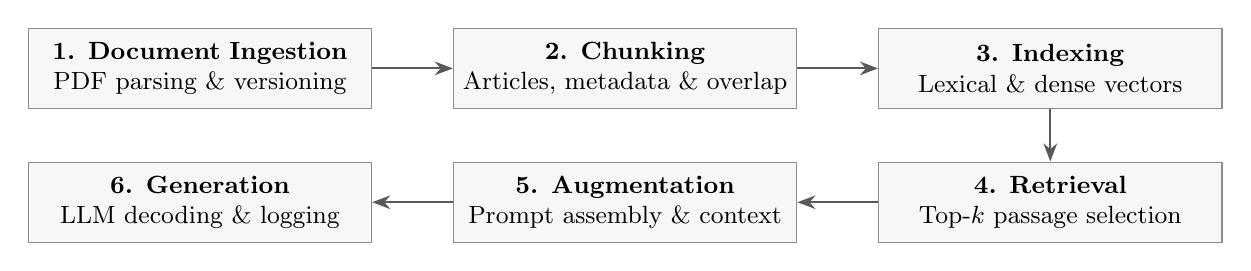
\begin{tikzpicture}[
  stage/.style={draw=black!45,fill=black!3,text width=4.15cm,
    minimum height=1.02cm,align=center,font=\small,inner sep=3pt},
  flow/.style={-{Stealth[length=2.3mm]},thick,draw=black!65}
]
\node[stage] (ingest) at (0,0) {\textbf{1. Document Ingestion}\\PDF parsing \& versioning};
\node[stage] (chunk) at (5.4,0) {\textbf{2. Chunking}\\Articles, metadata \& overlap};
\node[stage] (index) at (10.8,0) {\textbf{3. Indexing}\\Lexical \& dense vectors};
\node[stage] (retrieve) at (10.8,-1.7) {\textbf{4. Retrieval}\\Top-$k$ passage selection};
\node[stage] (prompt) at (5.4,-1.7) {\textbf{5. Augmentation}\\Prompt assembly \& context};
\node[stage] (generate) at (0,-1.7) {\textbf{6. Generation}\\LLM decoding \& logging};
\draw[flow] (ingest) -- (chunk);
\draw[flow] (chunk) -- (index);
\draw[flow] (index) -- (retrieve);
\draw[flow] (retrieve) -- (prompt);
\draw[flow] (prompt) -- (generate);
\end{tikzpicture}
\caption{RAG architecture and pipeline implementation (adapted from \cite{ref1}).}
\label{fig:pipeline}
\end{figure}

At the ingestion stage, OCR noise and table parsing errors can distort numerical data and conditional rules. During chunking, inappropriate boundary splits can detach core administrative conditions from regulatory articles. In indexing, versioning discrepancies may index obsolete clauses alongside active amendments. In retrieval, algorithms may miss critical clauses or prioritize topically adjacent distractor passages. In augmentation, truncating context windows can sever vital qualifying criteria. Finally, during generation, the model can misinterpret provided tabular data or hallucinate unsupported claims. Execution logs retain chunk IDs, context prompts, and completions to isolate failure stages.

\subsection{Three Retrieval Configurations}

TF-IDF represents passages via unigram and bigram token features scored using cosine similarity \cite{ref3}. BM25 incorporates word-segmented Vietnamese tokens and non-negative IDF, setting $k_1 = 1.5$ and $b = 0.75$ for term frequency saturation and document length normalization \cite{ref4}. BGE-M3 encodes queries and passages through its dense branch into normalized dense vectors ranked via cosine similarity \cite{ref5}. All three methods operate over identical chunk boundaries, queries, and ground-truth mapping rules.

\section{Evaluation Setup}

\subsection{Evaluation Metrics and Inference Parameters}

For query $q$ with $m$ gold evidence groups where $r$ groups appear in the top-$k$ retrieved candidates, Evidence Recall@$k(q) = r/m$. Binary metrics include $\text{Hit@}k(q) = 1$ if $r \ge 1$ and $\text{All Evidence Hit@}k(q) = 1$ if $r = m$. Metrics are macro-averaged across all 20 queries. Reciprocal rank $\text{MRR@}k$ uses the inverse rank of the first relevant evidence chunk, assigned 0 if no evidence appears within top-$k$. Chunks containing identical verbatim evidence clauses or repetitive headers are mapped to the same gold label.

Generation experiments evaluate $20 \text{ questions} \times 4 \text{ configurations} = 80 \text{ candidate answers}$. All configurations employ frozen \texttt{Qwen2.5-1.5B-Instruct} weights with greedy decoding, FP32 precision with SDPA attention, and a 768-token generation ceiling. The unaugmented baseline receives the query with an empty source block stating ``No external documents provided.'' The three RAG configurations receive the query augmented with top-5 retrieved passages. The system prompt instructs the model to rely strictly on provided sources, respect cohort applicability boundaries, report insufficient information where evidence is lacking, and cite source chunk IDs. Input prompts, context IDs, and raw completions are fully logged \cite{ref1,ref6}.

\subsection{Worked Example: Evidence Retrieval and Prompt Construction}

\textbf{Benchmark Query (Q01):} \emph{According to the 2026 Academic Regulations, how does a prerequisite course differ from a pre-learning course?}

\begin{table}[H]
\centering
\caption{Top-5 candidate passages retrieved by BGE-M3 for benchmark query Q01}
\label{tab:3}
\footnotesize
\begin{tabularx}{\textwidth}{>{\hsize=0.32\hsize\linewidth=\hsize\centering\arraybackslash}X>{\hsize=1.28\hsize\linewidth=\hsize\raggedright\arraybackslash}X>{\hsize=1.40\hsize\linewidth=\hsize\raggedright\arraybackslash}X}
\toprule
\textbf{Dense Rank} & \textbf{Chunk Identifier} & \textbf{Content Summary and Regulatory Scope} \\
\midrule
1 & \chunkid{D01_regulation_article_3_03} & Article 3, Clause 3(c), PDF page 4; contains definitions of both course types \\
2 & \chunkid{D01_regulation_article_27_01} & Article 27; transitional clauses for earlier cohorts \\
3 & \chunkid{D01_regulation_article_3_02} & Article 3, Clause 2; elective and general course definitions \\
4 & \chunkid{D01_regulation_article_6_02} & Article 6; semester scheduling and course planning \\
5 & \chunkid{D01_regulation_article_18_02} & Article 18; credit exemptions and transfer limits \\
\bottomrule
\end{tabularx}
\end{table}

Table~\ref{tab:3} lists the retrieval ranking from the BGE-M3 run. The prompt formats retrieved passages under a \texttt{SOURCES} header, displaying chunk IDs, titles, PDF page indices, and URLs. The rank-1 chunk explicitly defines prerequisite courses as requiring successful completion (passing) before enrolling in course A, whereas pre-learning courses merely require completing the study process.

\textbf{Grounded Model Response with Attribution:} To register and take course A, students must have completed and passed the prerequisite course. For a pre-learning course, the regulation requires students to have completed the study process prior to enrolling in course A. [\chunkid{D01_regulation_article_3_03}] \cite{ref7}

This grounded formulation reflects the semantic content generated by the dense embedding configuration. The model correctly articulated that prerequisite courses require ``passing'' whereas pre-learning courses require ``completing the study process.'' The citation identifier was verified and inserted during manual evaluation against Article 3, Clause 3(c). In contrast, the unaugmented baseline hallucinated generic definitions that omitted the decisive examination passing requirement.

\subsection{Response Quality Assessment Methodology}

Each generated response is evaluated against the gold answer, required key points, and corresponding regulatory articles across three qualitative tiers: Score 2 corresponds to fully correct core content, qualifying conditions, and numerical values; Score 1 corresponds to correct partial scope but misses secondary clauses; and Score 0 corresponds to incorrect conclusions or failure to provide an answer. The core factual accuracy rate is defined as the proportion of Score 2 answers across the 20 benchmark queries.

Unsupported or out-of-context claims are tracked via an independent binary flag. For instance, in query Q19, the TF-IDF configuration stated the correct regulatory timeline but hallucinated a non-existent decision suffix. Disconnecting core correctness from source attribution ensures that distinct error modes are tracked independently. Citation validity evaluates whether referenced chunk IDs exist within the prompt and directly ground the claim. Because all 60 RAG-generated answers omitted valid chunk IDs, citation rates are reported as zero.

Qualitative labels were assigned via automated GPT-based review conducted on 2026-11-08. The automated reviewer was unblinded to configuration labels, and scores are treated as provisional. While repository records confirm consistency checks on aggregate summary tables, independent double-blind human annotations for individual answers remain pending.

\subsection{Reproducibility and Experimental Artifacts}

To ensure complete experimental auditability, all datasets, segmentation pipelines, evaluation scripts, model generation logs, and review records are version-controlled in our open repository (\url{https://github.com/namkiet/CS420_SeminarRAG}). Specifically:
\begin{itemize}[leftmargin=*,itemsep=1pt,topsep=1pt]
\item \textbf{Retrieval Benchmark}: Automated runs across TF-IDF, BM25, and BGE-M3 correspond to commit \commitlink{5771d80}.
\item \textbf{Generation Benchmark}: 80 raw candidate completions across four experimental conditions are recorded at commit \commitlink{3bb5f3a}.
\item \textbf{Audit Trail and Verification}: Dataset sanity checks and review records are tracked at commit \commitlink{1182442}.
\end{itemize}

\section{Experimental Results}

\textbf{Retrieval Performance.} Table~\ref{tab:4} reports retrieval metrics across the 20 benchmark queries and 30 gold evidence groups. BM25 achieves superior precision in early ranks, leading Evidence Recall@1 (80.00\%) and MRR@5 (0.8667). Dense BGE-M3 demonstrates strong multi-passage coverage at higher cut-offs, achieving the highest Evidence Recall@5 (89.17\%) and Hit@5 (95.00\%). Expanding $k$ from 3 to 5 increases BGE-M3 recall by 7.50 percentage points, whereas lexical methods plateau. Nonetheless, both BM25 and BGE-M3 successfully capture complete evidence sets for 16 out of 20 queries at $k=5$.

\begin{table}[H]
\centering
\caption{Retrieval benchmark results across 20 evaluation queries}
\label{tab:4}
\footnotesize
\begin{tabularx}{\textwidth}{>{\hsize=1.05\hsize\linewidth=\hsize\raggedright\arraybackslash}X>{\hsize=1.20\hsize\linewidth=\hsize\centering\arraybackslash}X>{\hsize=0.90\hsize\linewidth=\hsize\centering\arraybackslash}X>{\hsize=0.90\hsize\linewidth=\hsize\centering\arraybackslash}X>{\hsize=0.80\hsize\linewidth=\hsize\centering\arraybackslash}X>{\hsize=1.15\hsize\linewidth=\hsize\centering\arraybackslash}X>{\hsize=1.00\hsize\linewidth=\hsize\centering\arraybackslash}X}
\toprule
\textbf{Retriever} & \textbf{Evidence Recall@1} & \textbf{Recall@3} & \textbf{Recall@5} & \textbf{Hit@5} & \textbf{All Evidence@5} & \textbf{MRR@5} \\
\midrule
TF-IDF & 70.83\% & 82.50\% & 82.50\% & 90.00\% & 15/20 & 0.8250 \\
BM25 & 80.00\% & 84.17\% & 84.17\% & 90.00\% & 16/20 & 0.8667 \\
BGE-M3 & 65.00\% & 81.67\% & 89.17\% & 95.00\% & 16/20 & 0.7867 \\
\bottomrule
\end{tabularx}
\end{table}

\textbf{Generation Quality.} Table~\ref{tab:5} summarizes answer quality across the 80 generation runs executed on an NVIDIA Tesla T4 GPU. The unaugmented baseline fails completely (0/20 correct), generating severe hallucinations on 15/20 questions and abstaining on the remaining 5. Incorporating RAG increases core accuracy to 50.00\% for TF-IDF and BGE-M3, and 45.00\% for BM25. Simultaneously, the rate of unsupported claims drops from 75.00\% (15/20) in the baseline to 40.00\% (TF-IDF), 35.00\% (BM25), and 30.00\% (BGE-M3).

\begin{table}[H]
\centering
\caption{Answer generation quality across 80 completions based on provisional review}
\label{tab:5}
\footnotesize
\begin{tabularx}{\textwidth}{>{\hsize=0.85\hsize\linewidth=\hsize\raggedright\arraybackslash}X>{\hsize=0.75\hsize\linewidth=\hsize\centering\arraybackslash}X>{\hsize=0.80\hsize\linewidth=\hsize\centering\arraybackslash}X>{\hsize=1.15\hsize\linewidth=\hsize\centering\arraybackslash}X>{\hsize=1.45\hsize\linewidth=\hsize\centering\arraybackslash}X}
\toprule
\textbf{Configuration} & \textbf{Fully Correct} & \textbf{Partially Correct} & \textbf{Incorrect / Unusable} & \textbf{Unsupported Claims} \\
\midrule
Baseline (No RAG) & 0/20 (0.0\%) & 3/20 (15.0\%) & 17/20 (85.0\%) & 15/20 (75.0\%) \\
RAG (TF-IDF) & 10/20 (50.0\%) & 5/20 (25.0\%) & 5/20 (25.0\%) & 8/20 (40.0\%) \\
RAG (BM25) & 9/20 (45.0\%) & 6/20 (30.0\%) & 5/20 (25.0\%) & 7/20 (35.0\%) \\
RAG (BGE-M3) & 10/20 (50.0\%) & 6/20 (30.0\%) & 4/20 (20.0\%) & 6/20 (30.0\%) \\
\bottomrule
\end{tabularx}
\end{table}

Despite achieving superior Evidence Recall@5 (89.17\%), BGE-M3 ties with TF-IDF on final answer accuracy (10/20). Crucially, all 60 RAG-augmented completions fail to produce formal in-text citation identifiers. These empirical observations establish that retrieval recall, factual synthesis, and citation grounding must be treated as interdependent yet distinct bottlenecks.

\section{Failure Analysis and Verification Mechanisms}

\begin{table}[H]
\centering
\caption{Five representative failure archetypes identified in generation logs}
\label{tab:6}
\footnotesize
\begin{tabularx}{\textwidth}{>{\hsize=0.28\hsize\linewidth=\hsize\raggedright\arraybackslash}X>{\hsize=1.42\hsize\linewidth=\hsize\raggedright\arraybackslash}X>{\hsize=1.30\hsize\linewidth=\hsize\raggedright\arraybackslash}X}
\toprule
\textbf{Query} & \textbf{Observed Prompt and Generation Behavior} & \textbf{Root Cause and Remediation Stage} \\
\midrule
Q07 & All three top-5 sets miss the 65--79 score band chunk. BGE-M3 fabricates ``Average 50 points'' for a 68-point input. & Retrieval omission of threshold clauses. Generator must flag missing evidence rather than guessing. \\
Q01 & The correct definition ranks first in all runs. TF-IDF and BM25 retrieve an English prerequisite chunk at rank 2, derailing generation. & Lexical distractor interference. Enforce semantic verification to confirm exact entity alignment. \\
Q05 & BGE-M3 receives Article 19 but asserts credit completion alone suffices for graduation. BM25 omits suspension criteria. & Generator condition pruning. Cross-reference generated criteria against regulatory checklists. \\
Q13 & All retrievers capture the tuition table and notes. BM25 and BGE-M3 read column C1 instead of C5. TF-IDF mislabels C1. & Tabular parsing failure. Explicitly map row-column intersections and compute verified arithmetic. \\
Q19 & TF-IDF captures valid deadlines but invents an erroneous decision suffix. BGE-M3 omits the 2-year validity window. & Source metadata hallucination and temporal omission. Validate source citations against verified registry. \\
\bottomrule
\end{tabularx}
\end{table}

Table~\ref{tab:6} reveals that errors originate at distinct pipeline junctures. Case Q07 illustrates retrieval failure, where the absence of relevant score thresholds triggers parametric speculation. Case Q01 demonstrates distractor sensitivity, where a topically adjacent lexical match misleads the generator. Cases Q05 and Q13 represent post-retrieval reasoning failures: the model overlooks critical conditions or misreads structured table columns despite gold evidence residing within the prompt. Case Q19 exhibits metadata hallucination. Crucially, runtime logs confirm that all selected chunks were successfully accommodated without exceeding the 768-token limit.

\textbf{Verification Mechanisms.} To mitigate post-retrieval hallucinations, responses should be decomposed into atomic tuples: $\langle\text{Claim}, \text{Condition}, \text{Chunk ID}, \text{Verbatim Quote}\rangle$. An automated verification engine can then execute three auditing passes: (i) validate that cited passage identifiers reside strictly within the active prompt context; (ii) align generated propositions against verbatim quotes using natural language inference (NLI); and (iii) verify administrative constraints (cohort years, degree programs, disciplinary status). For tabular queries, cell values must be mapped to explicit column headers and arithmetic differences computed deterministically. When evidence is incomplete, the system should trigger secondary retrieval or issue an explicit abstention, operationalizing GenXAI verification principles \cite{ref2}.

\textbf{Knowledge Base Maintenance.} To support corpus evolution, regulatory documents must be maintained within a structured version control registry capturing decision numbers, effective dates, amendment links, and SHA-256 hashes. When new circulars are enacted, an automated diff engine should identify invalidated chunks, update the vector index, and trigger regression benchmarks across dependent queries. Versioned query logs ensure auditability across temporal policy shifts.

\section{Limitations and Applicability Boundaries}

This investigation evaluates 51 pages across four regulatory documents from a single university. While representing a realistic administrative setting, this expands beyond the 5--10 page guideline suggested in the seminar topic specifications. All reported performance metrics reflect the full 51-page, 162-chunk corpus; scaling to larger cross-institutional repositories or divergent regulatory frameworks may introduce different retrieval dynamics.

The benchmark comprises 20 curated queries without an isolated held-out split; a single-query shift alters accuracy by 5.00 percentage points. Lacking statistical significance testing, configuration rankings should be interpreted cautiously. Furthermore, multi-clause questions introduce labeling nuances: scope metadata in chunk headers enabled the model to correctly resolve query Q14 even though the specific reference article was absent from top-5 candidates.

Measurement precision faces additional constraints: 29 corpus pages were OCR-processed without comprehensive token-level human auditing, and factual accuracy scores reflect automated GPT review without blinded human double-annotation. In addition, our setup did not isolate distractor volume, prompt phrasing, or model capacity; systematic ablation across generator scales remains future work. Context overhead imposes practical deployment trade-offs: average prompt length spans 2,749 to 3,205 tokens under RAG versus 236 tokens for the baseline. Expanding $k$ improves evidence recall but increases latency; pipeline selection must balance recall requirements against generator comprehension.

\section{Conclusion}

This empirical study on university academic regulations demonstrates that Retrieval-Augmented Generation substantially improves factual accuracy from 0\% in an unaugmented baseline to 45--50\% under top-5 retrieval. Lexical BM25 exhibits superior early-rank precision, while dense BGE-M3 maximizes aggregate evidence coverage at $k=5$. Nevertheless, external document grounding \emph{does not eliminate hallucinations}: generators frequently omit administrative conditions, misinterpret tabular data, and fail to output valid citation tags even when relevant evidence is present. These findings strongly support pairing retrieval pipelines with post-generation claim verification.

\textbf{AI Usage Declaration.} OpenAI Codex was employed to assist in drafting, structural organization, and LaTeX typesetting. GPT was utilized for provisional qualitative evaluation based on metadata schemas. All equations, numerical results, and error logs were independently verified against primary papers and version-controlled repository data. The authors accept full responsibility for all content and conclusions.

\clearpage
\begin{thebibliography}{99}
\small

\bibitem{ref1}
Lewis, P. et al. (2020). Retrieval-Augmented Generation for Knowledge-Intensive NLP Tasks. \emph{Advances in Neural Information Processing Systems (NeurIPS)}, 33, 9459--9474. \href{https://papers.neurips.cc/paper_files/paper/2020/hash/6b493230205f780e1bc26945df7481e5-Abstract.html}{Article}.

\bibitem{ref2}
Schneider, J. (2024). Explainable Generative AI (GenXAI): A survey, conceptualization, and research agenda. \emph{Artificial Intelligence Review}, 57, 289. \href{https://doi.org/10.1007/s10462-024-10916-x}{DOI: 10.1007/s10462-024-10916-x}.

\bibitem{ref3}
Salton, G. and Buckley, C. (1988). Term-weighting approaches in automatic text retrieval. \emph{Information Processing \& Management}, 24(5), 513--523. \href{https://doi.org/10.1016/0306-4573(88)90021-0}{DOI: 10.1016/0306-4573(88)90021-0}.

\bibitem{ref4}
Robertson, S. and Zaragoza, H. (2009). The Probabilistic Relevance Framework: BM25 and Beyond. \emph{Foundations and Trends in Information Retrieval}, 3(4), 333--389. \href{https://doi.org/10.1561/1500000019}{DOI: 10.1561/1500000019}.

\bibitem{ref5}
Chen, J. et al. (2024). M3-Embedding: Multi-Linguality, Multi-Functionality, Multi-Granularity Text Embeddings Through Self-Knowledge Distillation. \href{https://arxiv.org/abs/2402.03216}{arXiv: 2402.03216}.

\bibitem{ref6}
Qwen Team (2024). Qwen2.5 Technical Report. \href{https://arxiv.org/abs/2412.15115}{arXiv: 2412.15115}.

\bibitem{ref7}
VNU-HCM University of Science (2026). Undergraduate Academic Regulations, Decision 3087/QĐ-KHTN. \href{https://hcmus.edu.vn/quy-che-dao-tao-trinh-do-dai-hoc-nam-2026/}{Official Portal}.

\bibitem{ref8}
VNU-HCM University of Science. Regulations on Student Conduct Assessment 2020 \& Amendment 2023. \href{https://hcmus.edu.vn/quy-che-danh-gia-ket-qua-ren-luyen-sinh-vien-he-chinh-quy/}{Official Portal}. \href{https://github.com/namkiet/CS420_SeminarRAG/blob/3bb5f3a/experiment/data/raw/D02_quy_che_diem_ren_luyen_2020_sua_2023.pdf}{Archived PDF snapshot}.

\bibitem{ref9}
VNU-HCM University of Science (2026). Tuition Fee Schedule for Academic Year 2026--2027, Decision 3317/QĐ-KHTN. \href{https://hcmus.edu.vn/thong-bao-nop-hoc-phi-hoc-ky-1-2026-2027-chuong-trinh-dai-tra/}{Official Portal}. \href{https://github.com/namkiet/CS420_SeminarRAG/blob/3bb5f3a/experiment/data/raw/D03_hoc_phi_2026_2027_K2022_ve_sau.pdf}{Archived PDF snapshot}.

\bibitem{ref10}
VNU-HCM University of Science (2026). Foreign Language Proficiency and Graduation Exit Standards, Decision 2464/QĐ-KHTN. \href{https://hcmus.edu.vn/quy-dinh-ve-viec-hoc-ngoai-ngu-va-chuan-trinh-do-ngoai-ngu-khi-tot-nghiep-dai-hoc/}{Official Portal}. \href{https://github.com/namkiet/CS420_SeminarRAG/blob/3bb5f3a/experiment/data/raw/D04_chuan_ngoai_ngu_tot_nghiep_2026.pdf}{Archived PDF snapshot}.

\end{thebibliography}

\end{document}
